\chapter{Redes Neurais Artificiais} \label{cap:redes}

Comparado com os computadores mais avançados que existem hoje, o cérebro humano ainda se mostra muito mais poderoso e eficaz do que as máquinas. O cérebro é capaz de processar informação a uma velocidade muito maior do qualquer computador convencional e realiza com facilidade tarefas como o reconhecimento de padrões e classificação de objetos, enquanto algoritmos tradicionais falham. 

Redes neurais artificiais foram criadas com inspiração no funcionamento e na estrutura do cérebro, como uma alternativa poderosa para resolver problemas que as arquiteturas tradicionais não eram capazes de resolver eficientemente. Essas redes emulam a estrutura cerebral natural, se utilizando de elementos distintos de processamento (neurônios) que se comunicam para realizar a tarefa desejada. 

Simon Haykin\cite{Haykin} define uma rede neural como "...um processador distribuído massivamente paralelo composto por unidades simples de processamento, que possui uma propensidade natural a armazenar conhecimento experimental e torná-lo disponível para uso."

As redes neurais artificiais são utilizadas para resolver problemas como ajuste de funções, classificação de objetos e reconhecimento de padrões. Nesse capítulo, serão explicados conceitos importantes para o entendimento das redes artificiais, começando pelo seu elemento mais básico, o neurônio.

\section{Neurônios}

O neurônio é a estrutura básica do sistema nervoso central. É uma célula composta principalmente de três partes distintas: o corpo celular, os dendritos e o axônio. O corpo celular é a estrutra central do célula aonde está contido o núcleo do neurônio e são executados as suas funções vitais. Os dendritos são prolongamentos do corpo celular responsáveis por receber sinais e o axônio é uma extensão maior do corpo celular, responsável por enviar sinais a outros neurônios. Dois neurônios interagem em apenas  pontos de contato chamados sinapses. Nessas sinapses o axônio de um neurônio envia sinais para os dendritos de um segundo neurônio. A figura \ref{fig:neuronio} ilustra a estrutura básica dos neurônios.

\begin{figure}
\centering
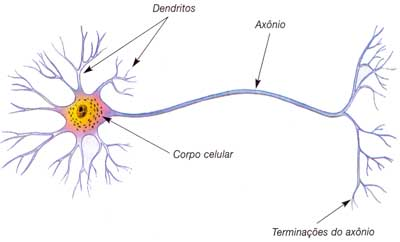
\includegraphics[width=.6\textwidth]{neuronio}
\label{fig:neuronio}
\caption{A estrutura básica de um neurônio humano}
\end{figure}

O neurônio artificial também possui três estruturas básicas semelhantes àquelas do neurônio natural. Seus três elementos básicos são: as entradas(análogas aos dendritos), a sáida(análoga ao axônio) e um núcleo de processamento. 

O neurônio pode ter uma ou mais conexões de entrada caracterizadas por um peso $wi$ e que recebe um valor $xi$. No núcleo do neurônio artificial há um somador que calcula o valor $u$ agregado das entradas, ponderadas pelo peso correspondente. O resultado dessa soma ponderada é então deslocado de um valor escalar e em seguida submetido a uma função chamada de função de ativação, que determina a saída final do neurônio. Em suma podemos descrever a saída de um neurônio $n$ que possui $i$ entradas através das seguintes equações:

\begin{equation}
 u_n = \sum_{j=1}^i x_jw_j
\end{equation}

\begin{equation}
s(n) = f(u_n + b)
\end{equation}

Aonde $u_n$ é o valor agregado das entradas, $x_j$ é a j-ésima entrada e $w_j$ o peso da conexão associada, $s(n)$ é a saída do neurônio, $f$ é a função de ativação e $b$ o deslocamento, ou $bias$ do neurônio $n$. A figura \ref{fig:neuroartificial} ilustra a estrutura básica de um neurônio artificial.

%imagem do neurônio artifical

Claramente, a função de ativação do neurônio é o grande fator que define o seu comportamento e consequentemente sua funcionalidade. Existem dois tipos básicos de funções de ativação\cite{Haykin}: a função degrau e a função sigmóide.

O neurônio mais simples possível tem sua saída regida por uma função degrau e saída binária. Isto é, se o valor agregado $u$ de suas entradas for maior que um determinado limiar, a sua saída será 1 e a saída será 0 caso contrário. Apesar de ser capaz de resolver alguns problemas, esse tipo de neurônio tem algumas desvantagens. Por vezes, alterações sutis podem representar a diferença entre os dois valores possíveis da sáida. Além disso, um alcance limitado de valores na saída prejudica o treinamento.

A escolha mais comum de de função de ativação para a construção de redes neurais é a família de funções sigmóides. Essas funções, que tem um gráfico com formato de \textit{S}, assumem valores contínuos entre 0 e 1, o que faz com que alterações sutis na entrada representem alterações mais sutis na saída, aumentando a qualidade da informação gerada pelo neurônio. A mais comum das funções sigmóides utilizadas é a função logística, definida pela equação \ref{eq:logistica}, onde $a$ é uma constante que mede a declividade da curva.

\begin{equation}

f(u) = \frac{1}{1 + \exp{-au}}

\label{eq:logistica}

\end{equation}

Um dos motivos que tornou a função logística uma escolha popular para os neurônios artificiais foi a sua derivação simples, uma vez que algoritmos de treinamento muitas vezes usam a derivada da função de ativação\cite{Kosabov}.

É interessante reparar que quando $a$ se aproxima do infinito, a função logística se comporta da mesma forma que a função degrau.

\begin{figure}
 \centering
\begin{subfigure}{.5\textwidth}
  \centering
  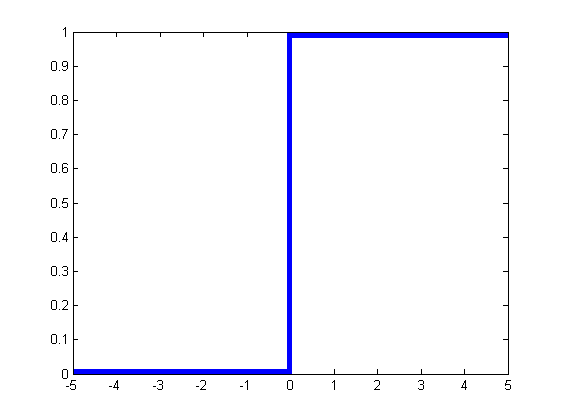
\includegraphics[width=.8\linewidth]{degrau}
	\caption{}
	\label{fig:ativacao:sub:degrau}
\end{subfigure}\
\begin{subfigure}{.5\textwidth}
  \centering
  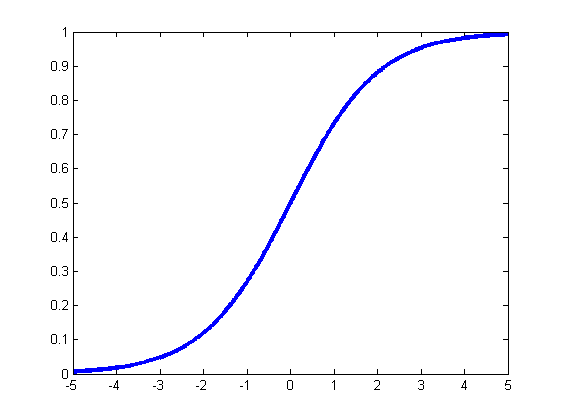
\includegraphics[width=.8\linewidth]{logistica}
	\caption{}
	\label{fig:ativacao:sub:logistica}
\end{subfigure}
\caption{(a) Gráfico da função degrau com limiar 0. (b) Gráfico da função logística com a = 1}
\label{fig:ativacao}
\end{figure}




\section{Redes Neurais Feed-Forward}


\section{Treinamento}

